%%%%%%%%%%%%%%%%%%%%%%%%%%%%%%%%%%%%%%%%%
% Beamer Presentation
% LaTeX Template
% Version 1.0 (10/11/12)
%
% This template has been downloaded from:
% http://www.LaTeXTemplates.com
%
% License:
% CC BY-NC-SA 3.0 (http://creativecommons.org/licenses/by-nc-sa/3.0/)
%
% Author:   Brigham H. Keys, Esq.
%%%%%%%%%%%%%%%%%%%%%%%%%%%%%%%%%%%%%%%%%

%----------------------------------------------------------------------------------------
%	PACKAGES AND THEMES
%----------------------------------------------------------------------------------------

\documentclass{beamer}

\mode<presentation> {

  %\usetheme{default}
  %\usetheme{AnnArbor}
  %\usetheme{Antibes}
  %\usetheme{Bergen}
  \usetheme{Berkeley}
  %\usetheme{Berlin}
  %\usetheme{Boadilla}
  %\usetheme{CambridgeUS}
  %\usetheme{Copenhagen}
  %\usetheme{Darmstadt}
  %\usetheme{Dresden}
  %\usetheme{Frankfurt}
  %\usetheme{Goettingen}
  %\usetheme{Hannover}
  %\usetheme{Ilmenau}
  %\usetheme{JuanLesPins}
  %\usetheme{Luebeck}
  %\usetheme{Madrid}
  %\usetheme{Malmoe}
  %\usetheme{Marburg}
  %\usetheme{Montpellier}
  %\usetheme{PaloAlto}
  %\usetheme{Pittsburgh}
  %\usetheme{Rochester}
  %\usetheme{Singapore}
  %\usetheme{Szeged}
  %\usetheme{Warsaw}

  % As well as themes, the Beamer class has a number of color themes
  % for any slide theme. Uncomment each of these in turn to see how it
  % changes the colors of your current slide theme.

  %\usecolortheme{albatross}
  %\usecolortheme{beaver}
  %\usecolortheme{beetle}
  %\usecolortheme{crane}
  %\usecolortheme{dolphin}
  %\usecolortheme{dove}
  %\usecolortheme{fly}
  %\usecolortheme{lily}
  %\usecolortheme{orchid}
  %\usecolortheme{rose}
  %\usecolortheme{seagull}
  %\usecolortheme{seahorse}
  %\usecolortheme{whale}
  %\usecolortheme{wolverine}

  %\setbeamertemplate{footline} % To remove the footer line in all slides uncomment this line
  %\setbeamertemplate{footline}[page number] % To replace the footer line in all slides with a simple slide count uncomment this line

  %\setbeamertemplate{navigation symbols}{} % To remove the navigation symbols from the bottom of all slides uncomment this line
}

\usepackage{graphicx} % Allows including images
\usepackage{booktabs} % Allows the use of \toprule, \midrule and \bottomrule in tables
\usepackage{multirow}

%----------------------------------------------------------------------------------------
%	TITLE PAGE
%----------------------------------------------------------------------------------------

\title[Hello Triangle]{Intro to Opengl} % The short title appears at the bottom of every slide, the full title is only on the title page

\author{Dane Christensen, Brigham H. Keys, Esq.} % Your name
\institute[BYU-I] % Your institution as it will appear on the bottom of every slide, may be shorthand to save space
          {
            BYU-Idaho \\ % Your institution for the title page
            \medskip
            \textit{key13005@byui.edu} % Your email address
          }
          \begin{document}

          \begin{frame}
            \titlepage % Print the title page as the first slide
            
\includegraphics[scale=.1]{logo.png}
          \end{frame}

          %\begin{frame}
          %\frametitle{Table of Contents} % Table of contents slide, comment this block out to remove it
          %\tableofcontents % Throughout your presentation, if you choose to use \section{} and \subsection{} commands, these will automatically be printed on this slide as an overview of your presentation
          %\end{frame}

          %----------------------------------------------------------------------------------------
          %	PRESENTATION SLIDES
          %----------------------------------------------------------------------------------------

          %------------------------------------------------
          \section{What is OpenGL?} % Sections can be created in order to organize your presentation into discrete blocks, all sections and subsections are automatically printed in the table of contents as an overview of the talk
          %------------------------------------------------

          %-------------BEGIN SLIDE------------------------
          \begin{frame}
            \frametitle{What is OpenGL?}
            OpenGL is the industry's foundation for high performance graphics, from games to virtual reality, mobile phones, and supercomputers. It is a cross-language, cross-platform application programming interface for rendering 2D and 3D vector graphics. The API is typically used to interact with a graphics processing unit (GPU), to achieve hardware-accelerated rendering. It does not handle windows, keyboard, mouse or any other kind of input from the user. However there are other APIs that work next to OpenGL to accomplish these tasks.
          \end{frame}
          %-------------END SLIDE--------------------------

          %-------------BEGIN SLIDE------------------------
          \subsection{History of OpenGL}
          \begin{frame}
            \frametitle{History of OpenGl}
            OpenGL has been out there for a while, with over 200 function and many legacy and deprecated functions. At the time of this writing the most up to date version of OpenGL is 4.5.
            \begin{scriptsize}
              \begin{itemize}
              \item 1980's -- Lacking an open standard, developers had to often write custom interfaces for each piece of hardware, this resulted in the duplication of effort and was largely inefficient.  
              \item Early 1990's -- Silicon Graphics was the leader of the 3D graphics for workstations. Their API called IRIS GL was the de facto industry standard. It's main competitor was the open standard named PHIGS. However IRIS GL was more popular because it was easier to use and it supported intermediate mode. However many companies such as IBM and Sun Microsystems were also pushing the PHIGS standard, offering extensions and weaking Silicon Graphics's market share. To combat this Silicon Graphics turned IRIS GL into an open standard called OpenGL.
              \item 1995 -- Microsoft released Direct 3D, which to this day is the main competitor to OpenGL.
              \item 2006 -- Control of the OpenGL API was transfered to the non-profit organization, the Khronos Group, who to this day control the API and many other open standards, some being WebGL and OpenGL ES.
              \item 2015 -- The Kronos Group announces the Vulkan API, a legacy free graphics API for next generation graphics.
              \end{itemize}
            \end{scriptsize}

          \end{frame}

          \section{Setting it up}
          \subsection{What am I going to need?}
          %-------------END SLIDE--------------------------

          %-------------BEGIN SLIDE------------------------
          \begin{frame}
            \frametitle{Libraries used in this course}
            \begin{block}{OpenGL}
              Chances are you already have the OpenGL installed as it is often bundled with your graphics card driver. However you likely are going to need to install the development files.
            \end{block}

            \begin{block}{The OpenGL Utility Library (GLU)}
              Is a collection of functions that do drawing on a higher level, and has functions that generally make our lives easier. It is bundled with OpenGL and uses OpenGL directly.
            \end{block}

            \begin{block}{FreeGlut}
              Another collection of functions that have high level drawing. But it's main purpose for us is to handle the keyboard, mouse and window handling. This will likely need to be installed.
            \end{block}
          \end{frame}
          %-------------END SLIDE--------------------------

          \subsection{Setting up the compiler}
          %-------------BEGIN SLIDE------------------------
          \begin{frame}
            \frametitle{Setting up the compiler}
            To compile code containing OpenGL functions, we need to let the compiler know that we are calling them in the first place by linking the libraries to our binary. Below are the individual flags we need to give to the compiler to use these utilities. Here is the syntax to compile the code from the command line:
            \begin{table}
              \begin{tabular}{l l l l l}
                \toprule
                \textbf{Compiler} & \textbf{File} & \textbf{OpenGL} & \textbf{GLU} & \textbf{FreeGlut}\\
                \midrule
                g++ & main.cpp & -lGL & -lGLU & -lglut \\
                \bottomrule
              \end{tabular}
            \end{table}
          \end{frame}
          %-------------END SLIDE--------------------------

          \subsection{Code}
          %-------------BEGIN SLIDE------------------------
          \begin{frame}
            \frametitle{Hello Triangle code}
            \begin{center}
              This code creates a triangle that looks like this:
              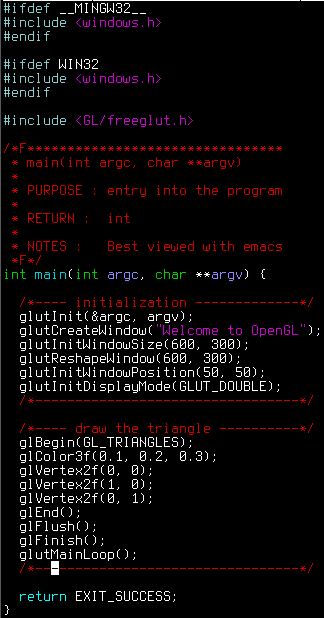
\includegraphics[scale=.33]{code.png}
              
\includegraphics[scale=.8]{result.png}
            \end{center}
          \end{frame}
          %-------------END SLIDE--------------------------

          \subsection{Other shapes we can draw}
          %-------------BEGIN SLIDE------------------------
          \begin{frame}
            \frametitle{Shapes we can draw}
            Triangles are one of the many things we can draw with the glBegin and glEnd functions, here is a list of a few things we can pass into glBegin and draw within minutes:\\
            \begin{itemize}
            \item{GL\_POINTS} -- A point is drawn for each call to glVertex.
            \item{GL\_LINES} -- Treats each pair of calls to glVertex as a line segment. At least 2 glVertex calls needed.
            \item{GL\_TRIANGLES} -- Treats each triplets of calls to glVertex as a triangle. At least 3 glVertex calls needed.  \item{GL\_QUADS} -- Treats each quartet of calls to glVertex as a quad. At least 4 glVertex calls needed.
            \item{GL\_POLYGON} -- Draws a single polygon with an arbitrary amount of sides. Unlike the other shapes every polygon requires it's own glBegin and glEnd, whereas you can draw multiple triangles with only one glBegin and glEnd.
            \end{itemize}
          \end{frame}
          %-------------END SLIDE--------------------------

          %-------------BEGIN SLIDE------------------------
          \begin{frame}
            \frametitle{References}
            \footnotesize{
              \begin{thebibliography}{99}
              \bibitem[Wikipedia, 2015]{p1} https://en.wikipedia.org/wiki/OpenGL (2015)

              \bibitem[OpenGL, 2015]{p1} https://www.opengl.org/ (2015)
              \end{thebibliography}
            }
            
\includegraphics[scale=.33]{cc.png}

          \end{frame}
          %-------------END SLIDE--------------------------

          %-------------END SHOW-------------------------------------------------------------------

          \end{document} 
